\documentclass[a4paper]{article}
\usepackage{amssymb}
\usepackage{amsmath}
\usepackage{hyperref}
\usepackage[italian]{cleveref}
\usepackage[autostyle=false, style=english]{csquotes}
\usepackage[italian]{babel}
%\usepackage[nomarkers]{endfloat}
\usepackage{graphicx}
\usepackage[margin=3cm]{geometry}
\usepackage{mathtools}
\usepackage{subcaption}
\usepackage[table]{xcolor}
%\renewcommand{\efloatseparator}{\mbox{}}
%\renewcommand{\efloatendlist}{\mbox{}}
\newenvironment{eqsys}{\begin{equation}\begin{dcases}}{\end{dcases}\end{equation}}
\graphicspath{{./images/}}
\MakeOuterQuote{"}

\DeclareMathOperator*{\sca}{\textrm{sca}}
\title{Progetto Controlli Automatici T \\ 1C - Controllo del posizionamento di un link flessibile}
\author{Riccardo Corradini \and Luigi di Nuzzo \and Kevin Michael Frick \and Davide Ragazzini \and Antony Zappacosta}
\begin{document}
\maketitle
\tableofcontents
\clearpage
\section{Descrizione e requisiti del sistema}
Nella nuova applicazione della azienda che commissiona il progetto si prevede di utilizzare una struttura meccanica particolarmente leggera. 
Questa però presenta il problema di una flessibilità non trascurabile intrinseca nei componenti meccanici utilizzati. 
Ciò rende difficile il posizionamento dell’estremità non attuata in una posizione fissa desiderata.
\subsection{Modello e linearizzazione}
L’intera struttura in questione è modellizzata dalla \cref{eqn:model} ed è schematizzata come in \cref{fig:sys_schem}.
\begin{eqsys}       
    \label{eqn:model}
    \dot{x_1}  =  f_1 (x_1, x_2, x_3, x_4)  =  x_2 \\
    \dot{x_2}  =  f_2 (x_1, x_2, x_3, x_4)  =  \frac{-M g L \sin (x_1) - K (x_1 - x_3) - \rho (x_2 - x_4)}{J} \\
    \dot{x_3}  =  f_3 (x_1, x_2, x_3, x_4)  =  x_4 \\
    \dot{x_4}  =  f_4 (x_1, x_2, x_3, x_4) + g(u)  =  \frac{K(x_1 - x_2) + \rho (x_2 - x_4) + u}{I}\\
    y  =  f_y (x_1, x_2, x_3, x_4)  =  x_1
\end{eqsys}
\begin{figure}[h!]
    \centering
 \begin{subfigure}{0.45\textwidth}
    \centering
    \includegraphics[width=\textwidth]{schematic.png}
    \caption{Schema del modello fisico del sistema.}
    \label{fig:sys_schem}
 \end{subfigure}
 ~
 \begin{subfigure}{0.45\textwidth}
    \centering
    \includegraphics[width=\textwidth]{control_sys.png}
    \caption{Schema di controllo del sistema linearizzato.}
    \label{fig:sys_cont}
 \end{subfigure}
\end{figure}
La variabile $\theta$ in \cref{fig:sys_schem} viene descritta dallo stato $x_1$ e rappresenta l’angolo rispetto ad un piano di riferimento fisso che la massa concentrata del link traccia nel suo moto. $\theta_m$ (nelle equazioni $x_3$) rappresenta l’angolo di rotazione del motore, il cui input $u$ al sistema è la coppia applicata $\tau_m$. $K, \rho, L, M_p, J_p, I$ sono rispettivamente: la costante elastica del link, il suo coefficiente di attrito dinamico, la lunghezza, la massa concentrata sull’estremità non attuata, il momento d’inerzia della stessa massa e il momento d’inerzia del link equivalente visto dal punto di vista del motore.
Ai fini dello sviluppo del controllo dell’impianto si vuole ottenere la struttura in \cref{fig:sys_cont}.

Come prima analisi il sistema non lineare è stato considerato nell’intorno di un punto di equilibrio, i cui valori $(\bar{x}, \bar{u})$ sono definiti nella \cref{table:ref_val}, e linearizzato nello stesso intorno servendosi della \cref{eqn:linearization_calc} ottenendo la \cref{eqn:linearization}.
Si è passato poi dalla rappresentazione nello spazio degli stati al dominio di Laplace utilizzando la trasformata di Laplace, ottenendo la funzione di trasferimento nella \cref{eqn:G}.

{\begin{table}[h!]

    \centering 

    \rowcolors{1}{gray!10}{gray!20}
    \begin{tabular}{| c | c || c | c |}
        
        $K$ & 3 &
        $\rho$ & 0.2 \\
        $L$ & 1 &
        $I$ & 0.01 \\
        $J_p$ & 0.02 &
        $M_p$ & 0.06 \\
        $\omega_n$ & 200 &
        $A_n$ & 0.05 \\
        $B_n$ & 20 &
        $h\%$ & 1 \\
        $T_{a_{h^\%}}$ & 0.8 &
        $W$ & $5^\circ$ \\
        $T_{a_o}$ & 0.4 &
        $\bar{u}$  & $M_p g L \sin(\bar{x_1})$ \\
        $\bar{x_1}$  & $\frac{\pi}{2}$ &
        $\bar{x_2}$  & 0 \\
        $\bar{x_3}$  &$\frac{\bar{u}}{K} + \bar{x_1}$ &
        $\bar{x_4}$  & 0
        
        
    \end{tabular}
    \caption{Specifiche del sistema.}
        \label{table:ref_val}
\end{table}
}
\begin{eqsys}       
        \nabla f_1  = (0, 1, 0, 0) \\
        \nabla f_2  = \frac{1}{J_p} (-M_p g L \cos(x_1) - K, - \rho, K, \rho) \\
        \nabla f_3  =  (0, 0, 0, 1)\\
        \nabla f_4  =  \frac{1}{I} (K, \rho, -K, -\rho) \\
        \nabla f_y  =  (1, 0, 0, 0)  \\
        \frac{dg}{du}  =  \frac{1}{I}
        \label{eqn:linearization_calc}
    \end{eqsys}

\begin{equation}
    \label{eqn:linearization}
A = \begin{pmatrix}0 & 1 & 0 & 0 \\
    -K/J_p & -\rho/J_p & K/J_p & \rho/J_p \\
    0    &   0    &   0    &   1\\
    K/I  & \rho/I & -K/I &-\rho/I
\end{pmatrix};
B = (0, 0, 0, \frac{1}{I})^T;
C = (1, 0, 0, 0);
D = (0);
\end{equation}



\begin{equation}
    \label{eqn:G}
    G(s) = \frac{1000 (s+15)}{s^2 (s^2 + 30s + 450)}
\end{equation}
Dopo aver definito su MATLAB i parametri del sistema, le matrici corrispondenti alla rappresentazione nello spazio degli stati del sistema linearizzato e la sua funzione di trasferimento, si è tracciato il diagramma di Bode del sistema in anello aperto, mostrato in \cref{fig:bode_G}, per $\omega \in [10^{-2}, 10^5]$.

\begin{figure}[h!]
    \centering
    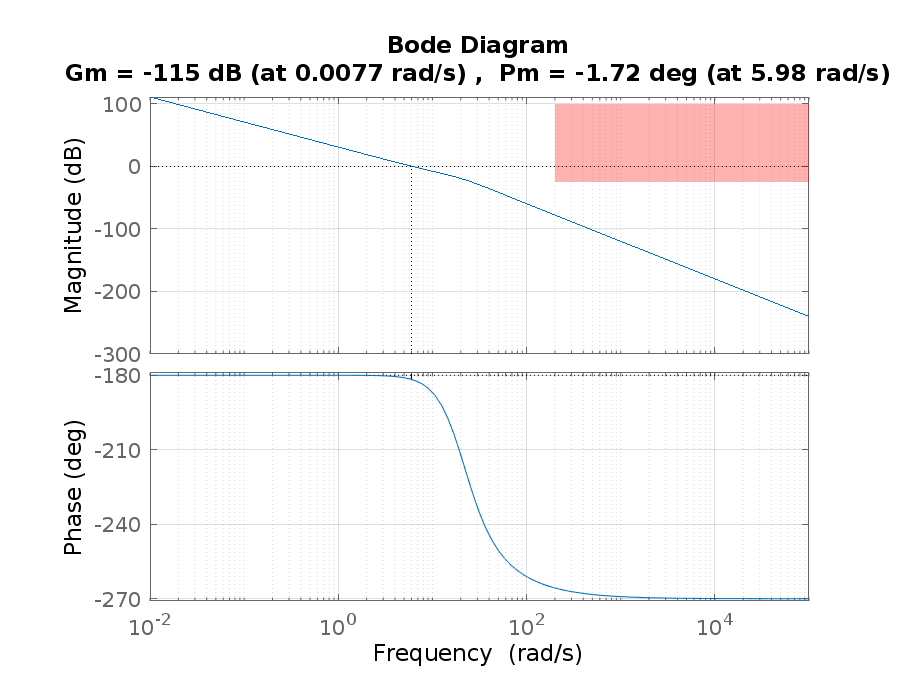
\includegraphics[width=\textwidth]{bode_G}
    \caption{Diagramma di Bode del sistema in anello aperto.}
    \label{fig:bode_G}
\end{figure}

\subsection{Specifiche}
Per l’applicazione che l’azienda ha in mente si devono rispettare per il sistema linearizzato determinate caratteristiche:
\begin{enumerate}
    \item Errore a regime nullo con riferimento a gradino con ampiezza $w(t) = W \sca(t)$.
    \item Margine di fase $\phi_m \geq 45^\circ$.
    \item Sovraelongazione percentuale $S\% \leq 1\%$.
    \item Tempo di assestamento all'1\% $T_{a1} = 0.8\hspace{0.3em} [s]$ (opzionalmente $0.4 \hspace{0.3em}[s]$).
    \item Abbattimento di 20 volte di un disturbo di misura che si fa sentire a $\omega_n > 200\hspace{0.3em} [rad/s]$ con ampiezza $A_n = 0.05$.
\end{enumerate}

\subsection{Requisiti sul margine di fase e sulla pulsazione critica}
Il requisito sulla sovraelongazione si traduce in un requisito sul margine di fase che è maggiore di quello specificato, indicato nella \cref{eqn:phim}.
Tuttavia, durante la sintesi del controllore si è notato che anche non rispettando questo requisito è possibile avere un sistema che rispetti le specifiche di sovraelongazione e abbia un tempo di assestamento ottimale.
Nei diagrammi di Bode l'intervallo che comprende fasi non accettabili, pur rispettando le specifiche sul tempo di assestamento e sull'abbattimento del rumore, è indicato in blu.

\begin{equation}
    \xi = \sqrt{\frac{\log(S_{max})^2}{(\pi^2+\log(S_{max})^2)}} \approx 0.826
    \label{eqn:xi}
\end{equation}

\begin{equation}
    \phi_m \approx \xi \cdot 100 \approx 83^\circ
    \label{eqn:phim}
\end{equation}

Il requisito sul tempo di assestamento si traduce invece in un requisito sulla pulsazione critica, che deve essere maggiore di una certa soglia indicata nella \cref{eqn:omega_c}.
Questa soglia è stata rispettata durante la sintesi del regolatore. 
Nei diagrammi di Bode le "zone proibite" che non rispettano i requisiti sono indicate in verde; le specifiche ottimali usano un colore meno intenso.
\begin{equation}
    \omega_c \gtrsim \frac{460}{\phi_m T_a} \approx 7 \hspace{0.3em} [rad/s] (\approx 14 \hspace{0.3em} [rad/s] \textrm{ per le specifiche ottimali})
    \label{eqn:omega_c}
\end{equation}

\section{Progetto del regolatore}

Per avere errore a regime nullo è necessario che $L(s)$ abbia un polo nell'origine, ma $G(s)$ ne ha due, che abbassano di molto la fase: si progetta quindi $R(s)$ in modo che abbia uno zero vicino all'origine che cancelli il polo.

Sono state progettati due regolatori: uno che rispetta le specifiche standard e uno, più complesso, che rispetta le specifiche ottimali.

\subsection{Specifiche standard}
Per rispettare le specifiche standard si è inserito uno zero nell'origine per cancellare un polo di $G(s)$ e avere un margine di fase pari ad almeno 83 gradi per pulsazioni critiche $\omega_c \le 10\hspace{0.3em} rad/s$.
Si è quindi cercato un guadagno che permettesse di rispettare tale pulsazione critica, dato dalla \cref{eqn:gain_sta}.
\begin{equation}
\mu_d =  10^{-\frac{1}{20}|(s \cdot G)(j \bar{\omega}_c)|_{dB}} \approx 0.25, \bar{\omega}_c = 9.5 \hspace{0.3em} [rad/s]
\label{eqn:gain_sta}
\end{equation}
Si è quindi inserito un polo a cinque decadi dall'origine per garantire la fisica realizzabilità.

\subsection{Specifiche ottimali}
Il regolatore che rispetta le specifiche opzionali si serve di due reti anticipatrici, una con punto medio in $\omega_1 = 1/ (T_1 \sqrt{\alpha_1}) = 0.132 \hspace{0.3em} [rad/s]$ e un'altra con punto medio in $\omega_2 = 1/ (T_2 \sqrt{\alpha_2}) \approx 2.7 \cdot 10^{-2} \hspace{0.3em} [rad/s]$.
La prima rete anticipatrice ha una larghezza di banda di circa quattro decadi, con uno zero a $\omega_{z1} \approx -0.06 \hspace{0.3em} [rad/s]$ e un polo a $\omega_{p1} \approx -10^3 \hspace{0.3em} [rad/s]$. 
La seconda rete anticipatrice ha una larghezza di banda di meno di una decade, con uno zero a $\omega_{z2} \approx -20\hspace{0.3em} [rad/s]$ e un polo a $\omega_{p2} \approx -70\hspace{0.3em} [rad/s]$.

I parametri delle reti anticipatrici sono $T_1 = 17.42\hspace{0.3em} [rad/s], \alpha_1 = 5.741 \cdot 10^{-5}, T_2 = 0.05\hspace{0.3em} [rad/s], \alpha_2 = 0.286$.
La seconda rete anticipatrice ha il polo e lo zero più vicini tra loro per evitare di aumentare troppo l'ampiezza e rispettare le specifiche sull'abbattimento del rumore.

Il guadagno di questo regolatore è $\mu_d = 3.4 \cdot 10^{-2}$.

La funzione di trasferimento del regolatore standard è data dalla \cref{eqn:R_sta}, mentre quella del regolatore più complesso è data dalla \cref{eqn:R_opt}.
I diagrammi di Bode sono mostrati rispetrivamente in \cref{fig:bode_L_sta} e in \cref{fig:bode_L}.
\begin{equation}
    \label{eqn:R_sta}
    R_{sta}(s) = \frac{ 0.2456 s}{ 1+  10^{-5} s}
\end{equation}
\begin{equation}
    \label{eqn:R_opt}
    R_{opt}(s) = \frac{0.02961 s^2 + 0.594 s + 0.034}{ 1.43 \cdot 10^{-5} s^2 + 0.0153 s + 1}
\end{equation}

\begin{figure}[h!]
    \centering
    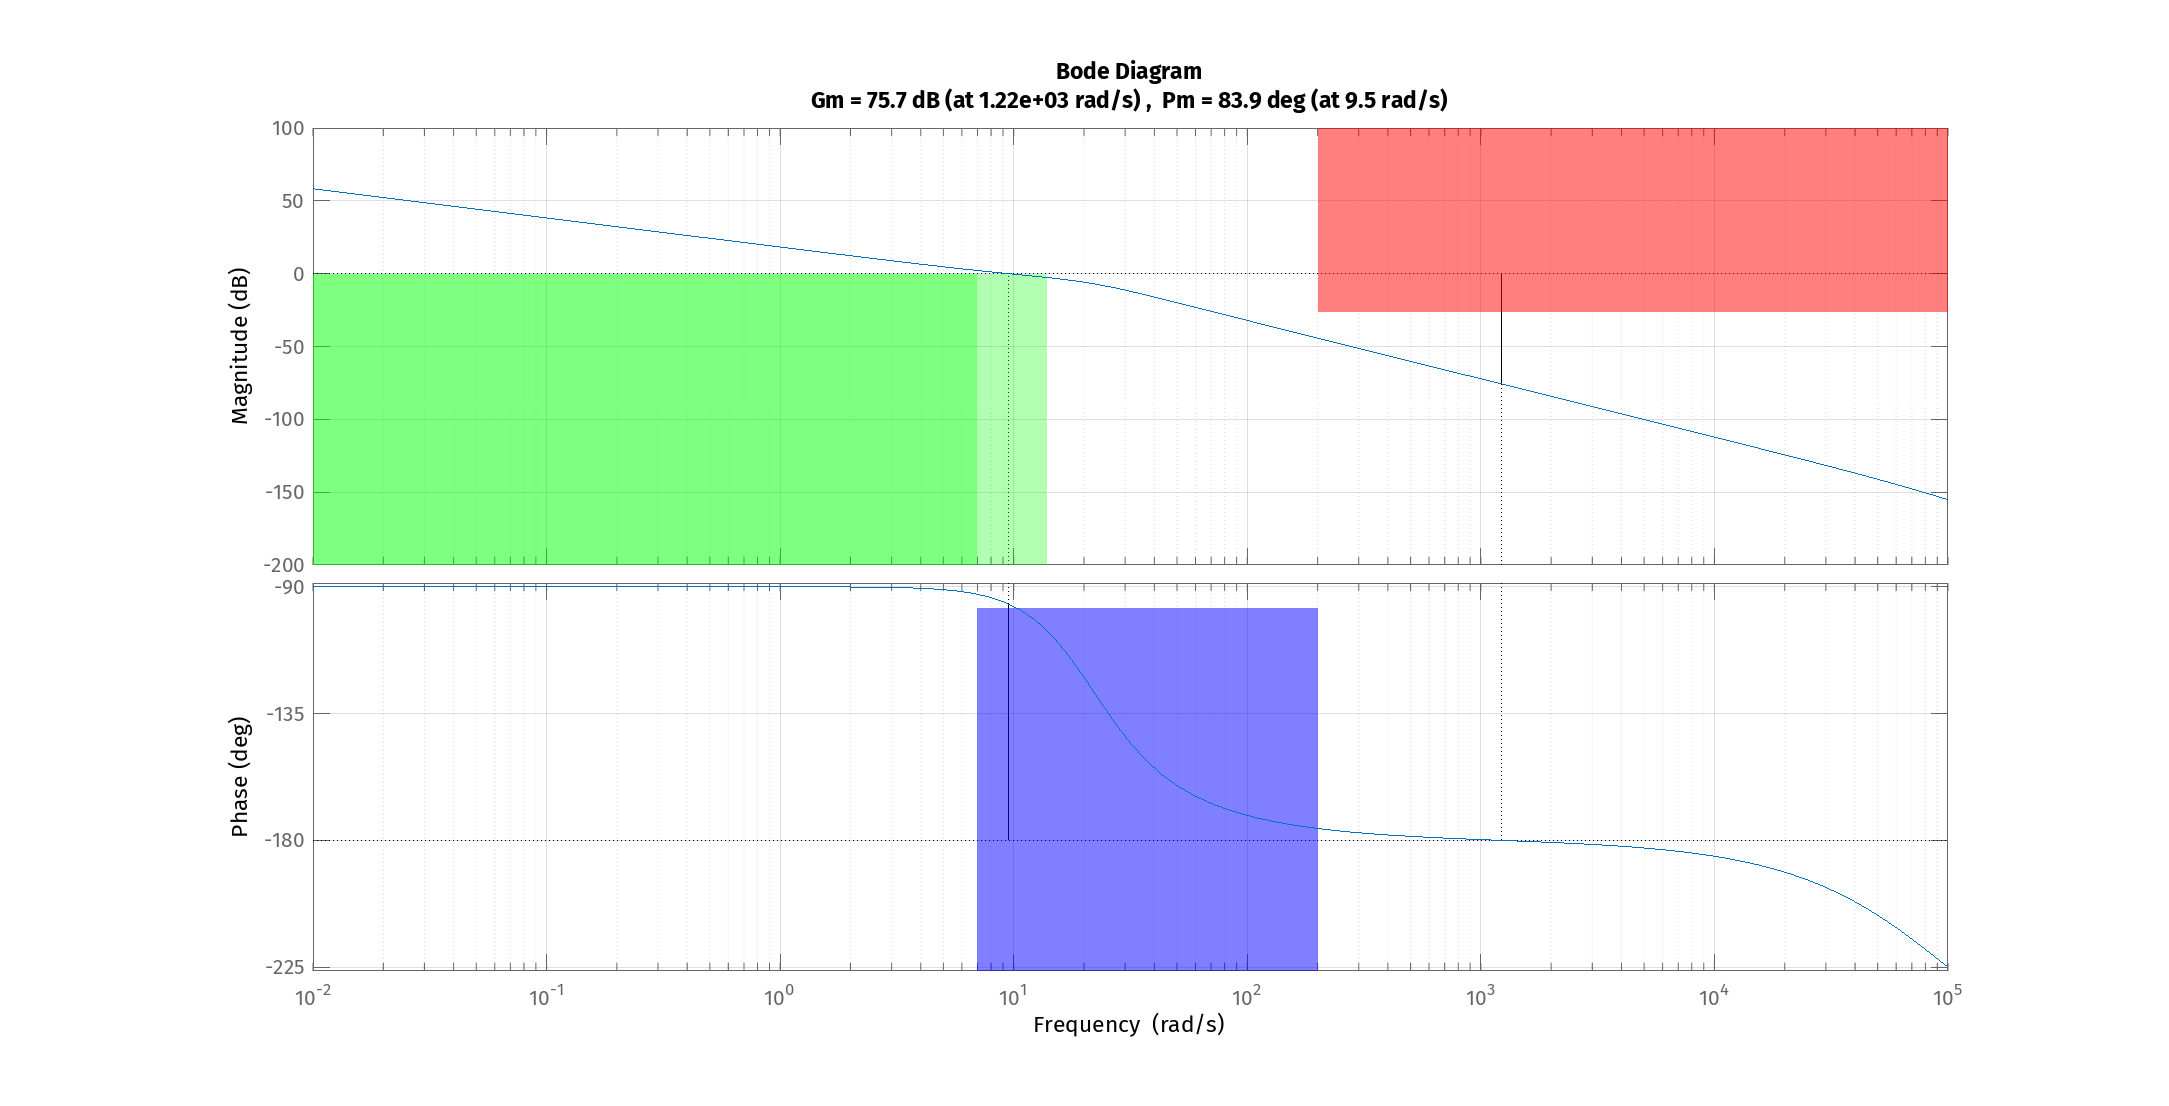
\includegraphics[width=\textwidth]{bode_L_sta}
    \caption{Diagramma di Bode del sistema con regolatore che rispetta le specifiche standard.}
    \label{fig:bode_L_sta}
\end{figure}

\begin{figure}[h!]
    \centering
    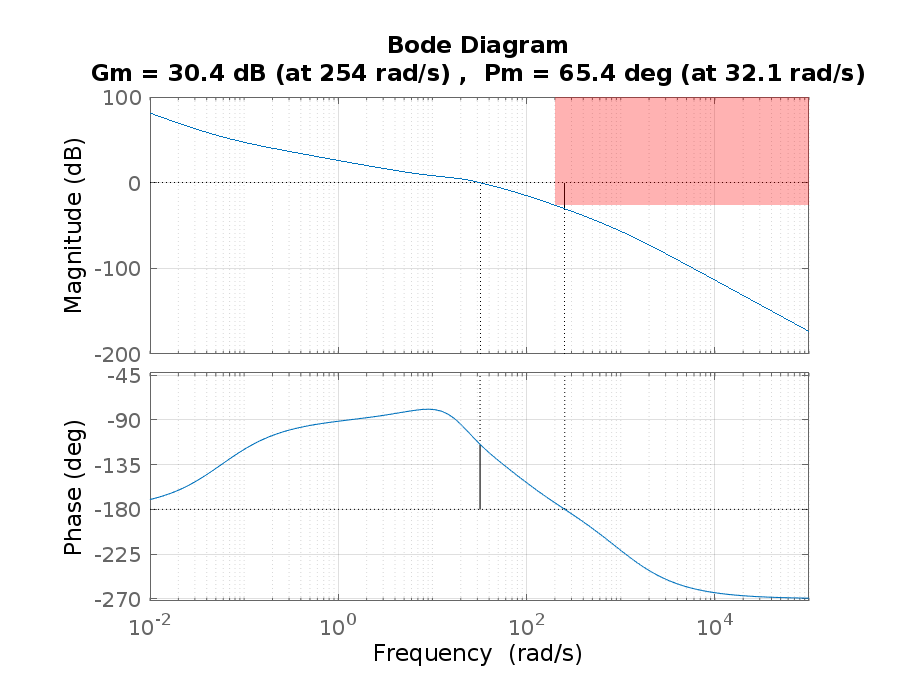
\includegraphics[width=\textwidth]{bode_L}
    \caption{Diagramma di Bode del sistema con regolatore che rispetta le specifiche ottimali.}
    \label{fig:bode_L}
\end{figure}

\section{Risposta del sistema in anello chiuso con regolatore}
Il regolatore standard non presenta sovraelongazione quando applicato al sistema linearizzato, mentre quello ottimale presenta una sovraelongazione percentuale dello 0.23\% circa, rispettando le specifiche.
Il regolatore semplice garantisce un tempo di assestamento all'1\% pari a 0.5045 secondi, mentre il regolatore ottimale garantisce un tempo di assestamento all'1\% pari a 0.3817 secondi (misurato con la funzione MATLAB \texttt{stepinfo}).
\begin{figure}[h!]
    \centering
    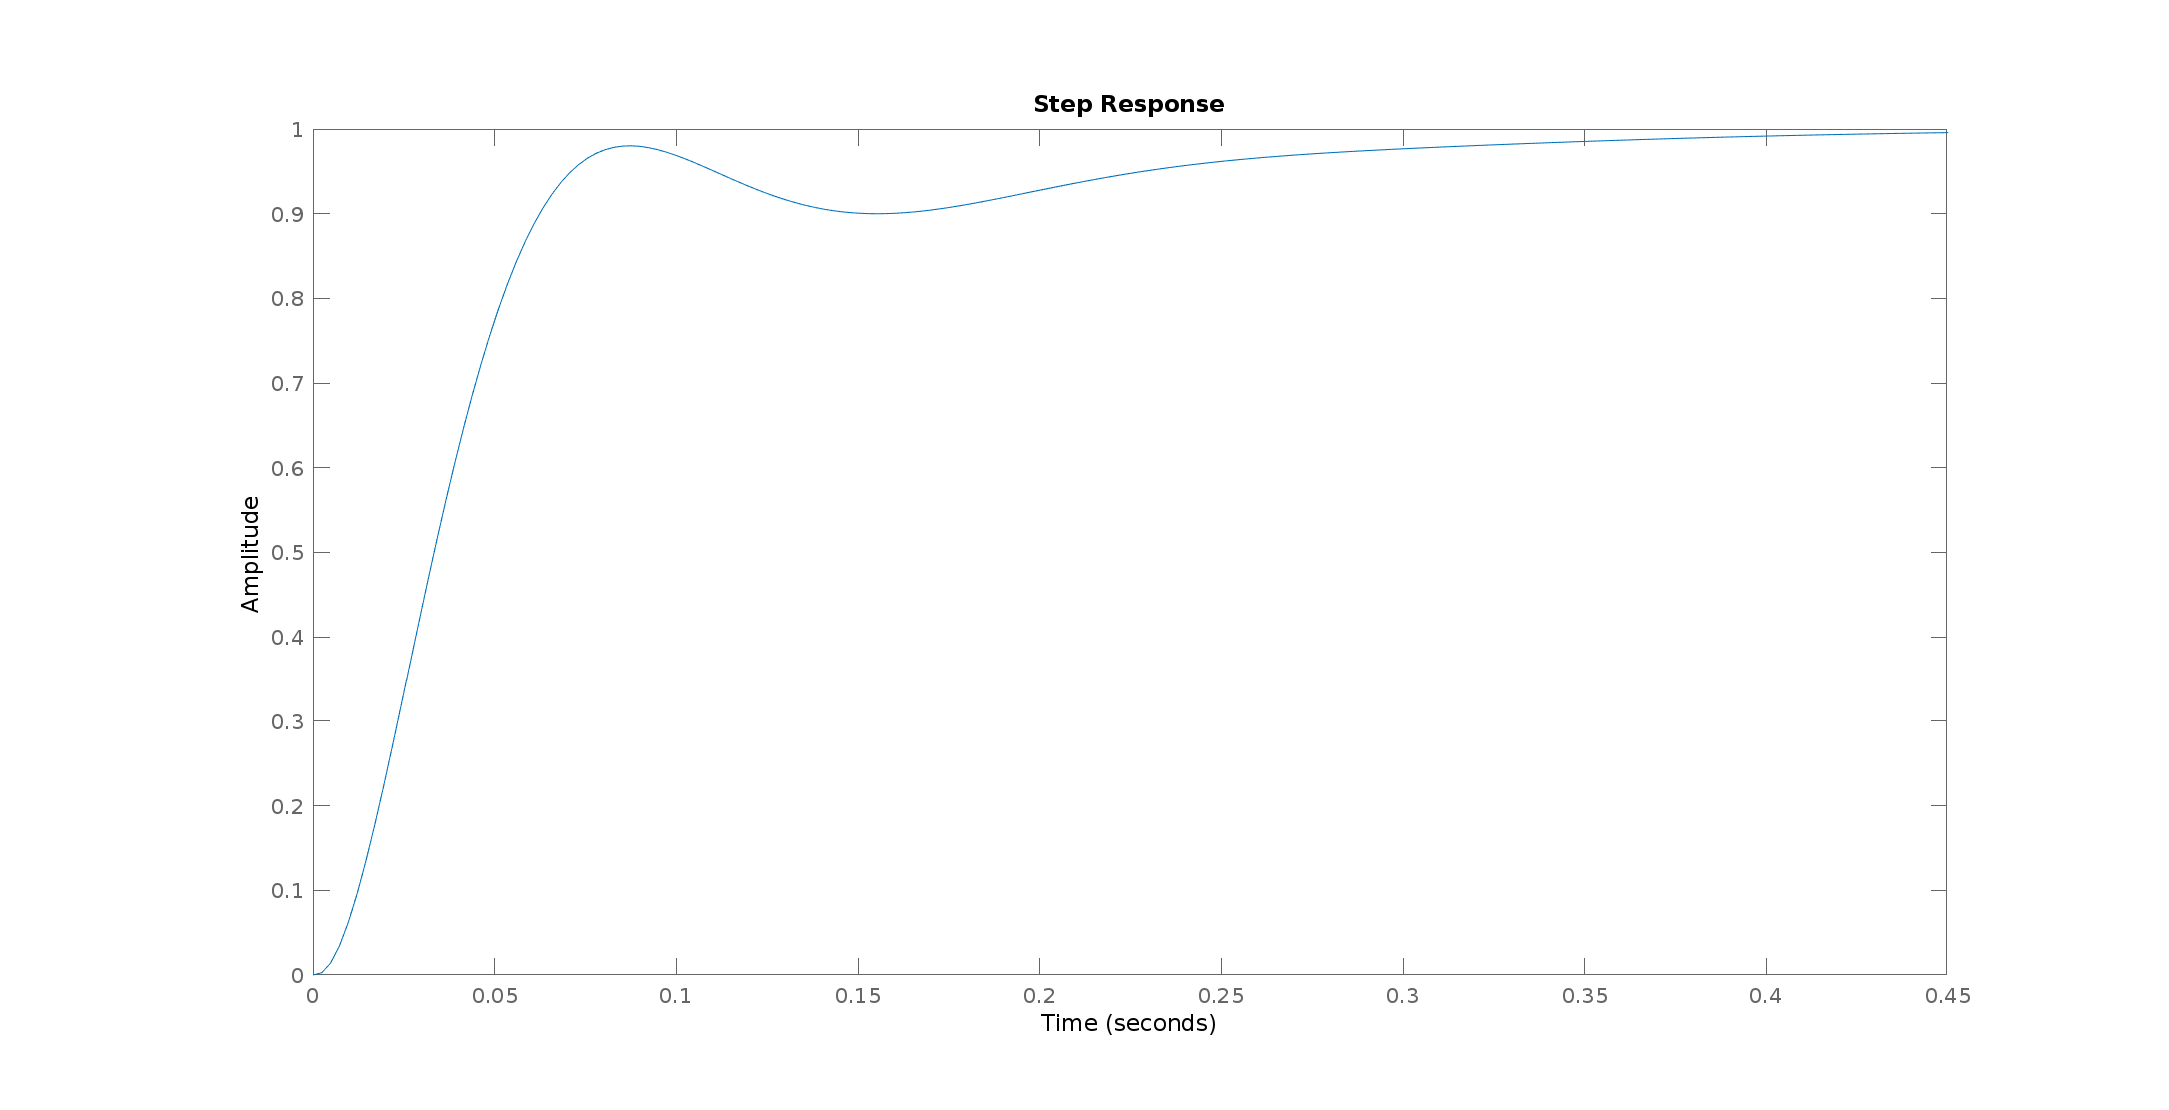
\includegraphics[width=0.8\textwidth]{step_opt}
    \caption{Risposta allo scalino del sistema in anello chiuso con regolatore ottimale.}
    \label{fig:step_opt}
    \end{figure}
\begin{figure}[h!]
    \centering
    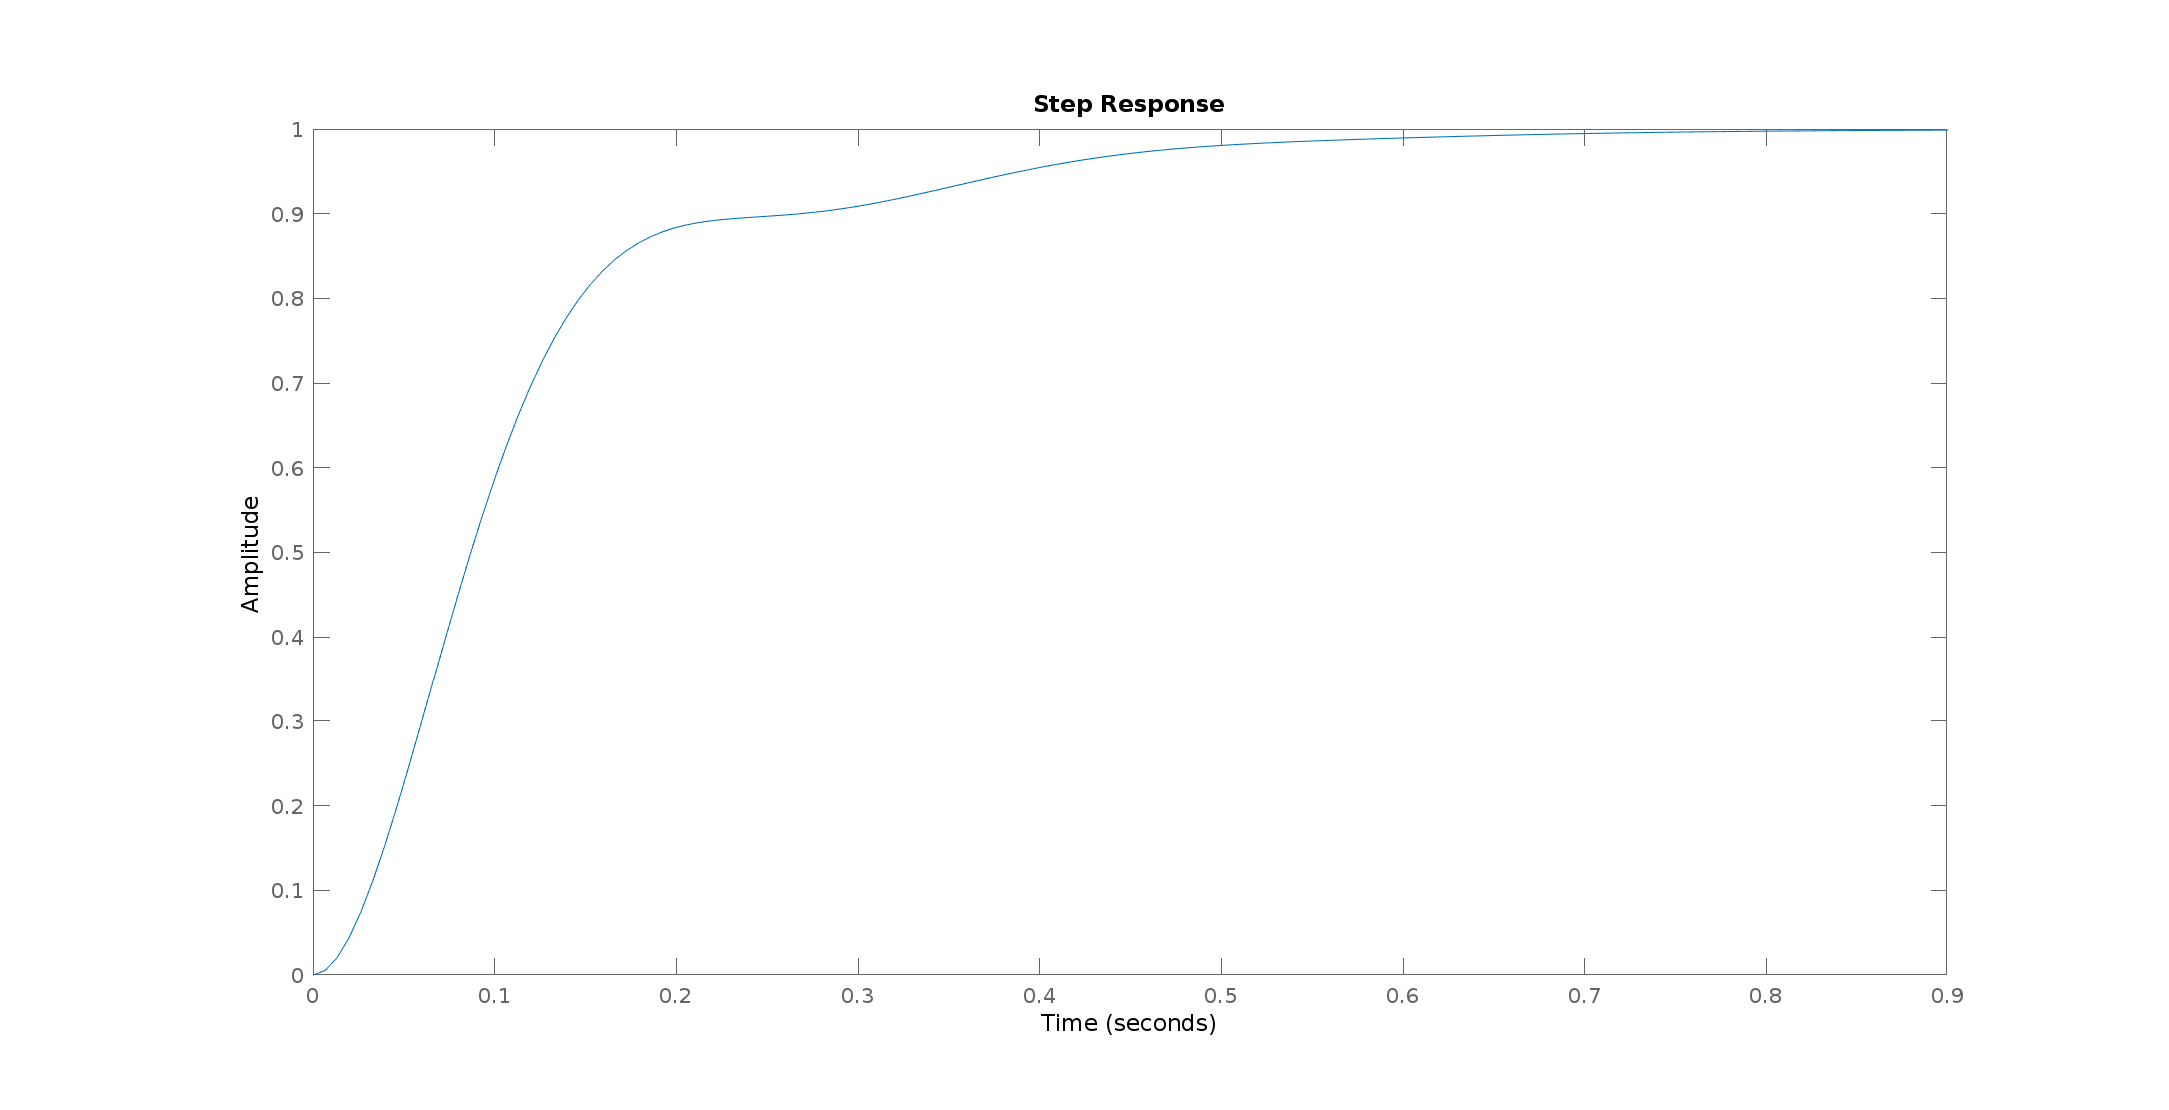
\includegraphics[width=0.8\textwidth]{step_sta}
    \caption{Risposta allo scalino del sistema in anello chiuso con regolatore standard.}
    \label{fig:step_sta}
\end{figure}

\subsection{Studio del luogo delle radici}
Dallo studio del luogo delle radici mostrato in \cref{fig:rlocus} si evince che i poli nell'origine tendono a diventare complessi coniugati a parte reale positiva per valori alti della costante di trasferimento. 
Ciò significa che aumentando il guadagno o inserendo zeri reali o poli complessi coniugati ad alte frequenze il sistema diventa instabile.
Con il regolatore progettato, tuttavia, il guadagno non è abbastanza alto perché ciò accada.

\begin{figure}[h!]
    \centering
    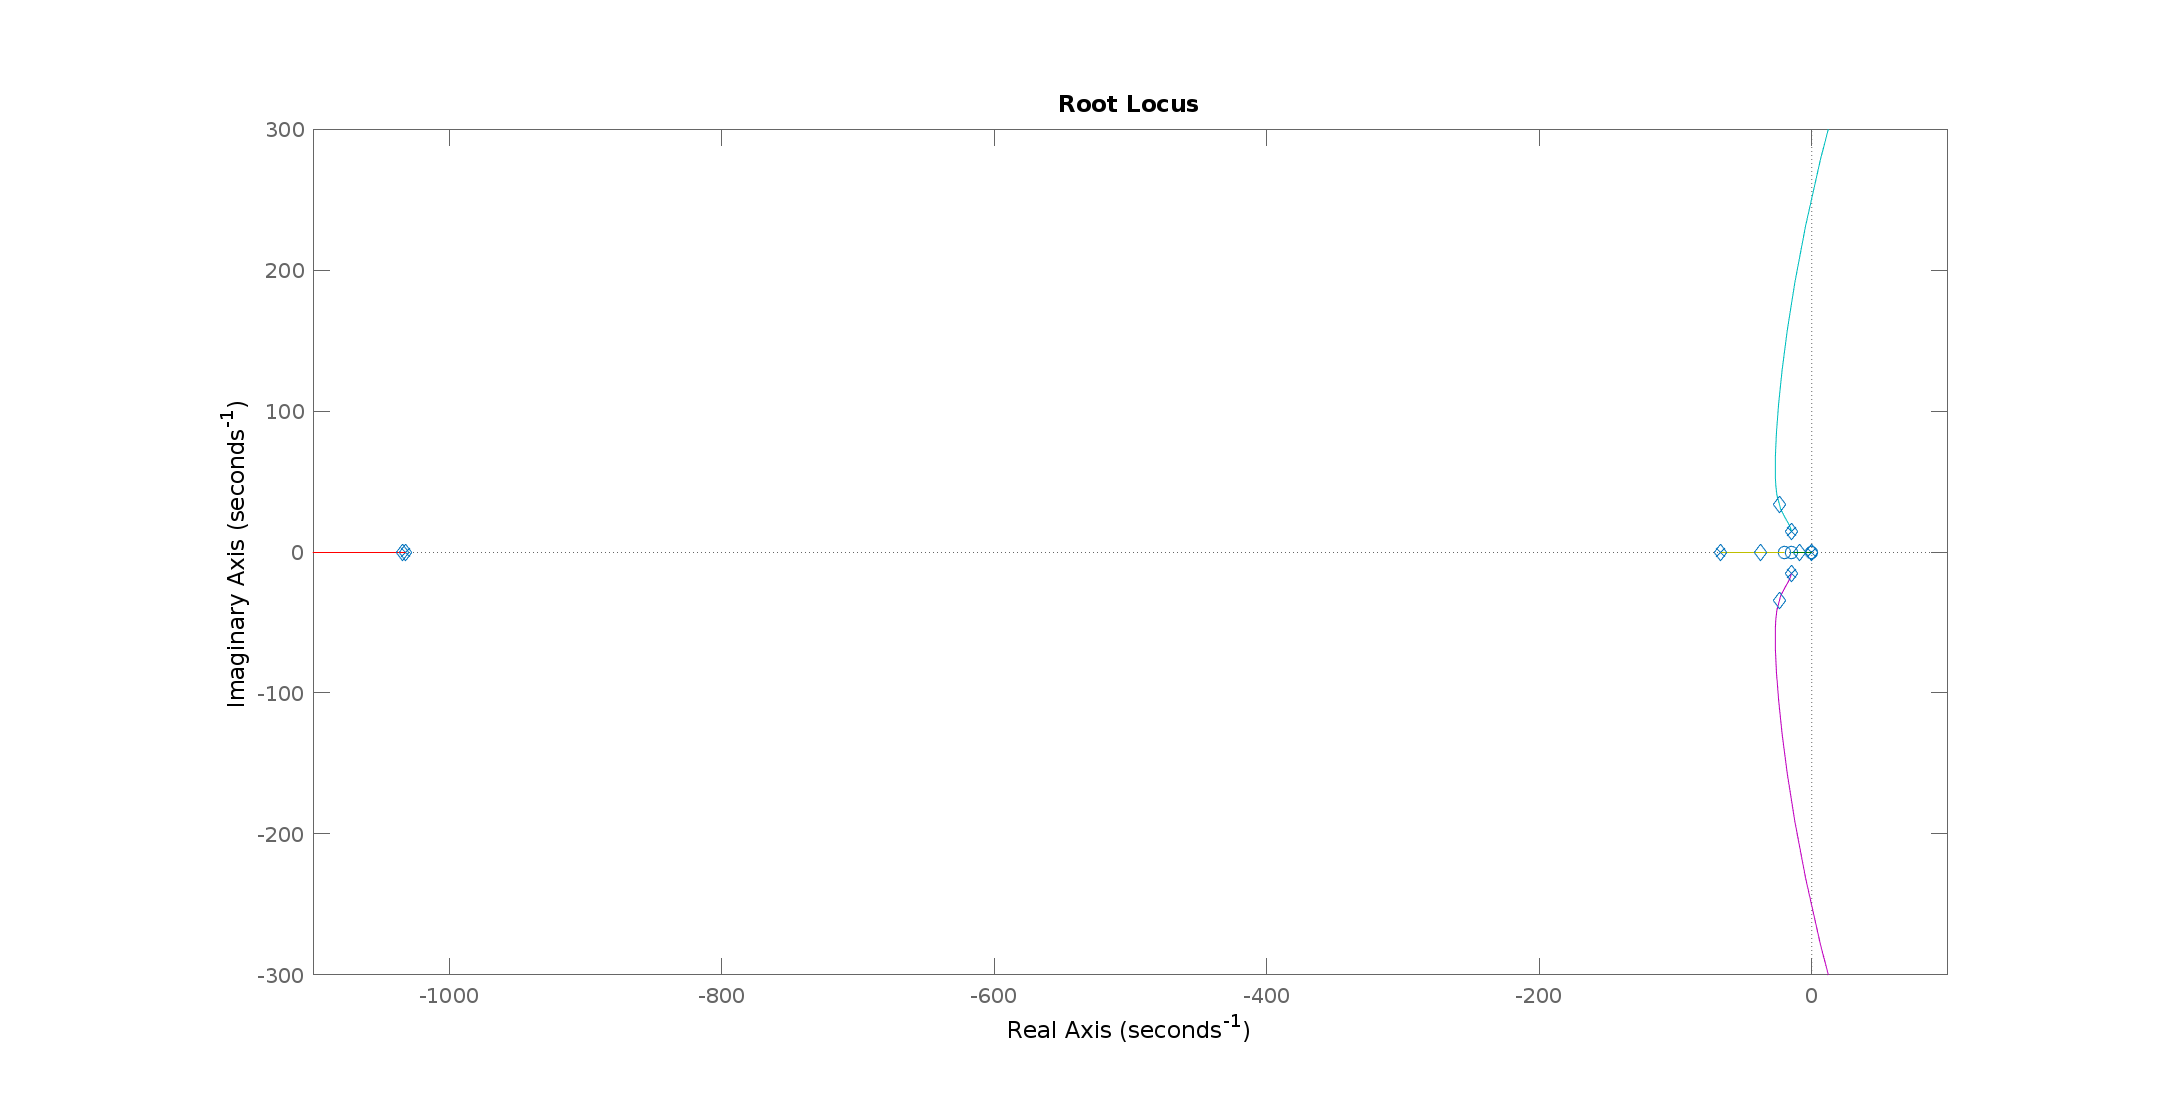
\includegraphics[width=0.65\textwidth]{rlocus}
    \caption{Luogo delle radici del sistema con regolatore ottimale.}
    \label{fig:rlocus}
\end{figure}

\subsection{Simulink}
Il sistema è stato simulato, sia nella sua versione linearizzata che in quella non linearizzata, servendosi del pacchetto software Simulink. 
Il sistema non linearizzato è stato realizzato con un blocco "MATLAB Function" che calcola le espressioni nella \cref{eqn:model}, le passa a quattro blocchi integratori e riceve in ingresso il risultato.
Il regolatore ottimale riesce a ottenere buone prestazioni, evidenziate nelle \cref{fig:sim_nonlin} e \cref{fig:step_sim_nonlin}, anche nel sistema non linearizzato.
Si osserva tuttavia che quest'ultimo presenta notevoli divergenze dal sistema linearizzato per i valori di ingresso a scalino richiesti dalle specifiche, rimanendo stabile solo con sollecitazioni almeno otto volte meno intense.
\begin{figure}[h!]
    \centering
    \includegraphics[width=0.7\textwidth]{Simul1C.pdf}
    \caption{Schema Simulink del sistema linearizzato.}
    \label{fig:sim_lin}
\end{figure}
\begin{figure}[h!]
    \centering
    \includegraphics[width=0.7\textwidth]{NonLin1C.pdf}
    \caption{Schema Simulink del sistema non linearizzato. }
    \label{fig:sim_nonlin}
\end{figure}
La risposta allo scalino del sistema linearizzato ricalca quella ottenuta con la funzione \texttt{step} di MATLAB.
La risposta allo scalino del sistema non linearizzato mostra che è possibile ottenere stabilità solamente con valori di ingresso a scalino inferiori a $w = \frac{W}{8} \sca(t)$. 
\begin{figure}[h!]
    \centering
\begin{subfigure}[t]{0.48\textwidth}
    \centering
    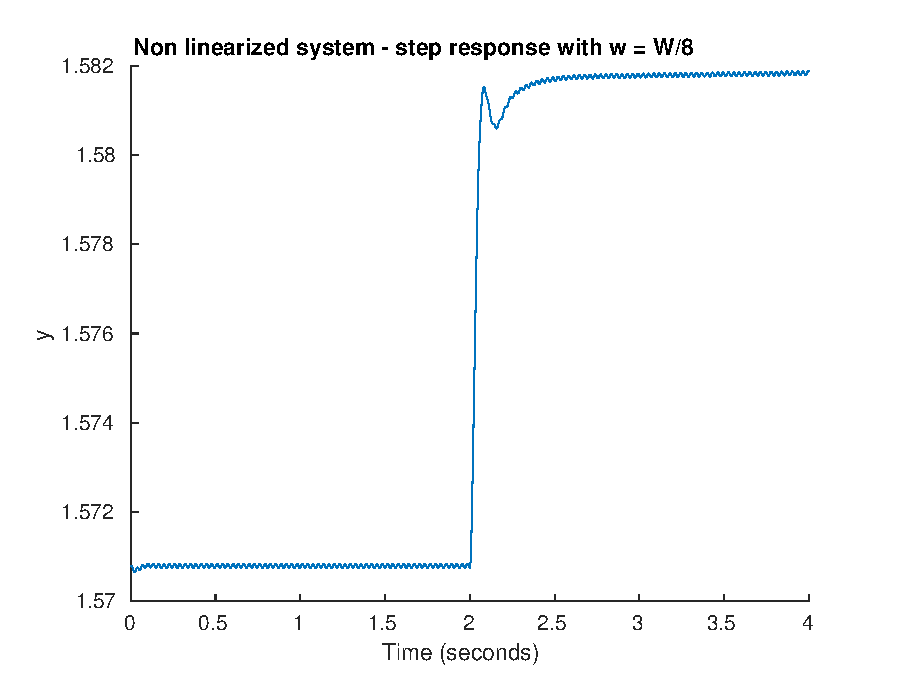
\includegraphics[width=\textwidth]{step_nonlin_short}
    \caption{Risposta allo scalino del sistema non linearizzato con ingresso $w = \frac{W}{8} \sca (t)$.}
    \label{fig:step_sim_nonlin}
\end{subfigure}
~
\begin{subfigure}[t]{0.48\textwidth}
    \centering
    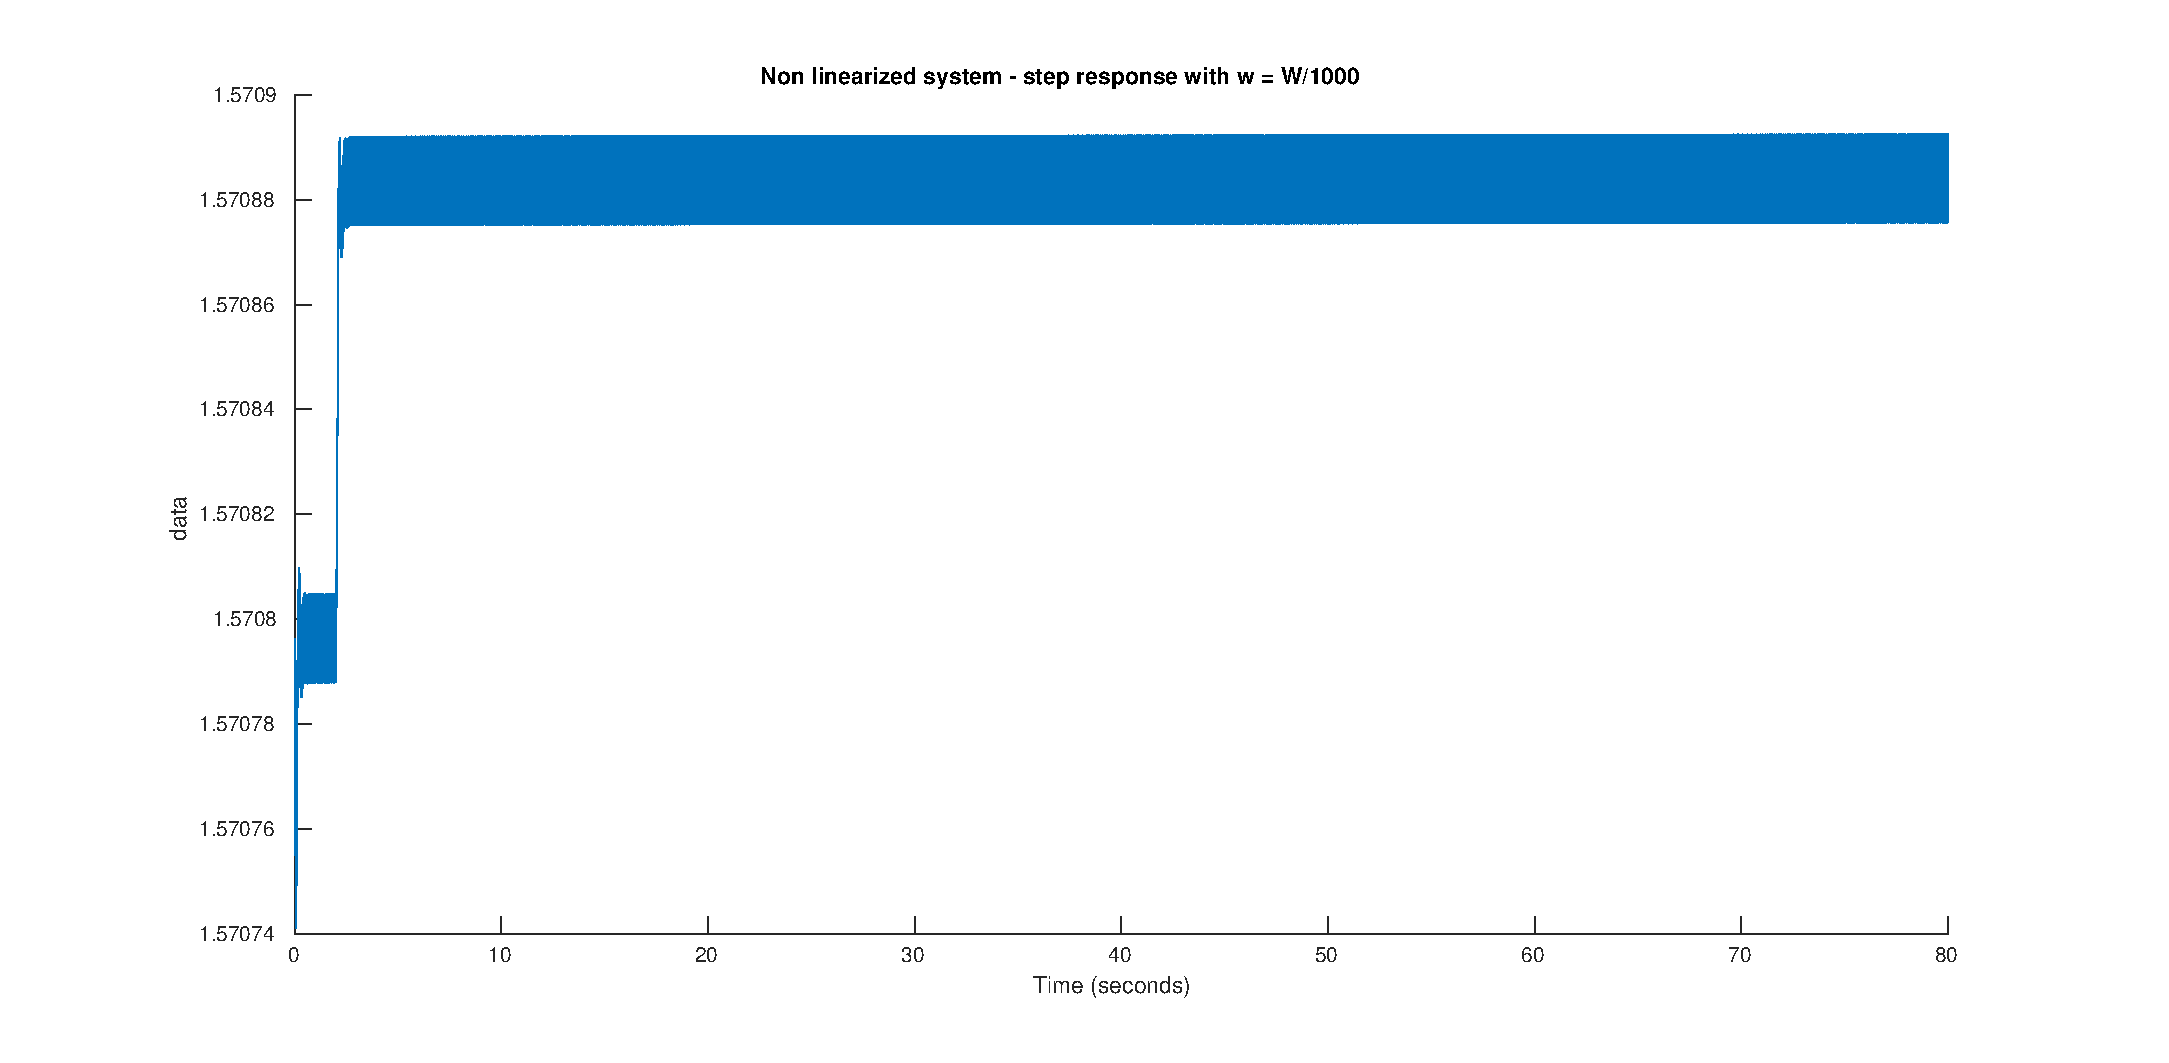
\includegraphics[width=\textwidth]{step_nonlin_long}
    \caption{Risposta allo scalino del sistema non linearizzato con ingresso $w = \frac{W}{8} \sca (t)$ che mostra la lunga coda di assestamento.}
    \label{fig:step_sim_nonlin_long}
\end{subfigure}
\end{figure}
\begin{figure}
\centering
\begin{subfigure}[t]{0.48\textwidth}
    \centering
    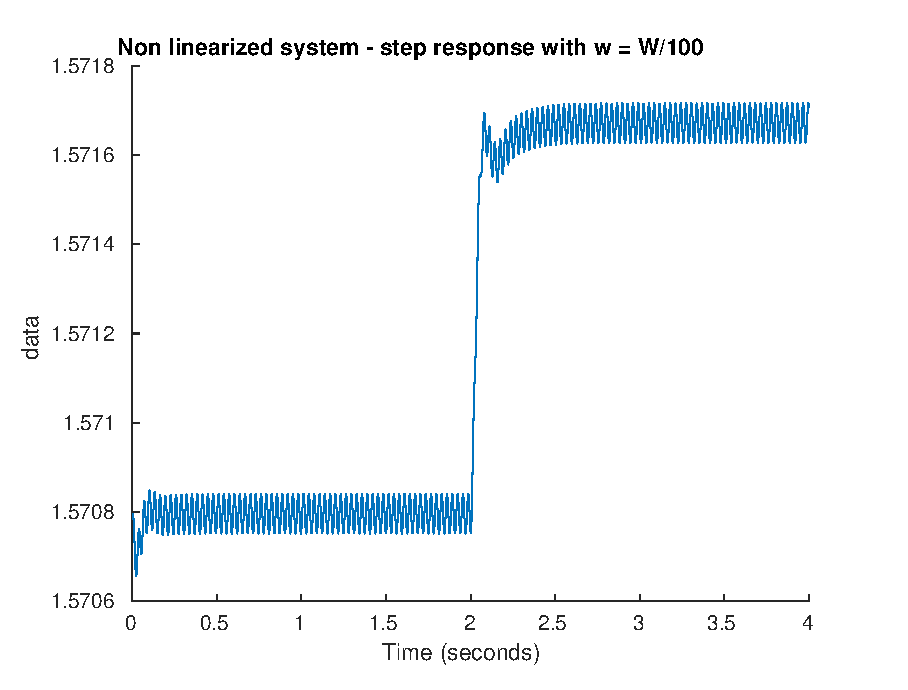
\includegraphics[width=\textwidth]{step_small_nonlin_short}
    \caption{Risposta allo scalino del sistema non linearizzato con ingresso $w = \frac{W}{100} \sca (t)$.}
    \label{fig:step_small_sim_nonlin_short}
\end{subfigure}
~
\begin{subfigure}[t]{0.48\textwidth}
    \centering
    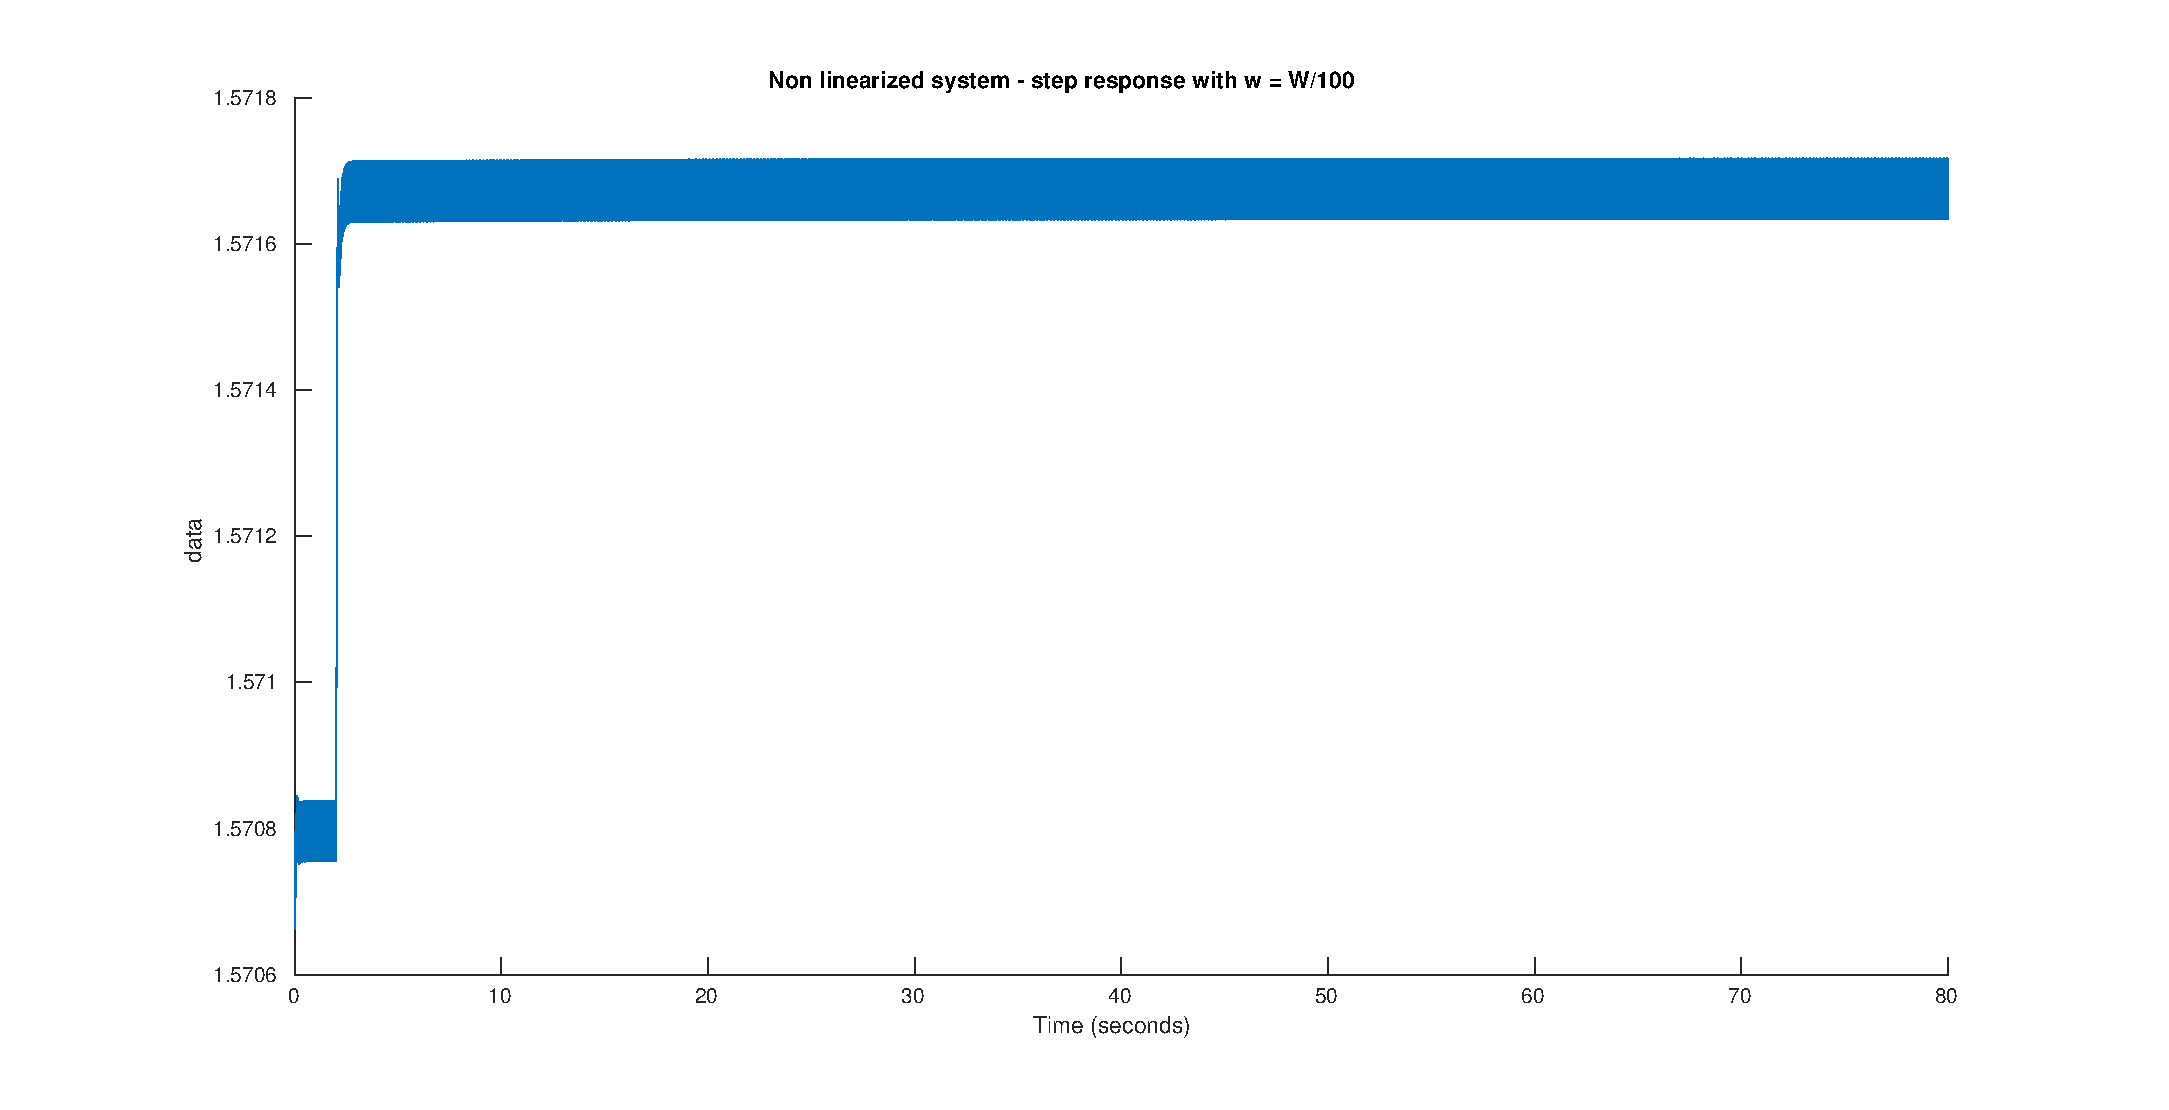
\includegraphics[width=\textwidth]{step_small_nonlin_long}
    \caption{Risposta allo scalino del sistema non linearizzato con ingresso $w = \frac{W}{100} \sca (t)$. La coda di assestamento non è osservabile per ingressi più piccoli.}
    \label{fig:step_small_sim_nonlin_long}
\end{subfigure}
\end{figure}
\section{Conclusioni}
Nonostante le ottime prestazioni che il regolatore ottimale riesce a raggiungere sul sistema linearizzato, il sistema reale è resistente solo a sollecitazioni otto volte minori del riferimento e, come mostrato nella \cref{fig:step_sim_nonlin_long}, presenta code di assestamento molto lunghe che non si osservano solo con sollecitazioni cento volte minori del riferimento (si veda la \cref{fig:step_small_sim_nonlin_long}). 
Le specifiche sulla sovraelongazione sembrano richiedere un margine di fase più ampio di quello fornito dal regolatore ottimale, nondimeno si osserva come quest'ultimo presenti una sovraelongazione percentuale che rispetta i requisiti.
Queste criticità mettono in evidenza l'entità delle approssimazioni utilizzate durante la sintesi del sistema di controllo e dovrebbero essere portate all'attenzione dell'azienda che commissiona il progetto e attentamente esaminate prima della fisica realizzazione e installazione del regolatore.
\end{document}
